\documentclass[11pt,a4paper]{article}
\usepackage[margin=2.4cm]{geometry}
\usepackage{graphicx,booktabs,amsmath,natbib,hyperref,xcolor}
\usepackage[T1]{fontenc}
\hypersetup{colorlinks=true,linkcolor=blue!55!black,citecolor=blue!55!black,urlcolor=blue!55!black}
\graphicspath{{../plots/}}
\newcommand{\masyr}{mas\,yr$^{-1}$}
\newcommand{\kms}{km\,s$^{-1}$}
\newcommand{\ocen}{$\omega$\,Cen}
\title{\ocen: kinematic data preparation for the dark-matter inference}
\author{oCen\_dm project notes}
\date{2026 September 19}

\begin{document}
\maketitle

\begin{abstract}
This note documents how the proper-motion and line-of-sight dispersion profiles that enter
the \ocen\ mass inference were assembled: which catalogues, which quality selections, which
estimator, and which cross-checks. The central methodological point is that both major
proper-motion catalogues contain a large population of stars whose quoted uncertainties are
underestimated, and that any dispersion measured from them is a statement about the error
model rather than about the cluster. Once each survey's own quality selection is respected,
HST and \emph{Gaia}~EDR3 agree to $0\pm4$ per cent in their overlap, an independent
Pristine-based measurement agrees with \emph{Gaia} to $0.5\pm1.4$ per cent, and both
published profiles are reproduced to a few tenths of a per cent. The final dataset is 127
binned points from five profiles spanning $0.05$--$57$\,pc.
\end{abstract}

\section{Scope and principle}

The inference asks whether \ocen\ requires a dark component beyond its stars and remnants.
That question is decided in the outskirts, where a halo would raise the dispersion above what
the luminous mass supports. The outskirts are also where the data are worst. Every
methodological choice below follows from a single principle, which we arrived at
independently and later found stated explicitly by \citet{haeberle2025}:

\begin{quote}
A star whose measurement uncertainty approaches the velocity dispersion being measured makes
the inferred dispersion a function of the assumed error model rather than of the cluster.
\end{quote}

Such stars are therefore excluded rather than modelled.

\section{Data sources}

\begin{table}[h]
\centering
\small
\begin{tabular}{llll}
\toprule
Dataset & Source & Content & Role \\
\midrule
oMEGACat VI & \citet{haeberle2025} & $1.48\times10^6$ HST PMs to $466''$ & primary inner PM \\
oMEGACat I / MUSE & \citet{haeberle2025} & $3\times10^5$ LOS velocities & inner LOS \\
\emph{Gaia} EDR3 members & \citet{vasiliev2021} & $2.28\times10^5$ stars to $0.67^\circ$ & primary outer PM \\
\emph{Gaia} DR2 profile & \citet{baumgardt2019} & 9 binned points & outer PM, published \\
Pristine periphery & \citet{kuzma2025} & $1.57\times10^5$ stars to $5.1^\circ$ & external check \\
Periphery spectroscopy & \citet{kuzma2026} & 592 LOS velocities to $3.15^\circ$ & external check \\
\bottomrule
\end{tabular}
\caption{Catalogues used. Only the first four enter the likelihood.}
\end{table}

\section{The dispersion estimator}
\label{sec:estimator}

All profiles measured in this project use the same estimator, applied per annulus.

\paragraph{Model.} Each star contributes a two-component mixture. The cluster is a
two-dimensional Gaussian whose principal axes follow that star's own radial direction,
\begin{equation}
\mathsf{C}_i = R(\phi_i)\,\mathrm{diag}(\sigma_R^2,\sigma_T^2)\,R(\phi_i)^{\!\top}
              + \mathsf{E}_i + \mathsf{D}_i ,
\end{equation}
with $\mathsf{E}_i$ the star's full proper-motion error covariance, including the
correlation coefficient, and $\mathsf{D}_i$ a rank-one term for the apparent dispersion
induced by the cluster's line-of-sight depth. The field is an \emph{empirical}
two-dimensional proper-motion density measured outside the cluster, not a Gaussian. The free
parameters per annulus are $\sigma_R$, $\sigma_T$, the two mean motions, and the field
fraction.

\paragraph{Why two dimensions.} Projecting the field onto each star's radial direction mixes
its two unequal widths ($3.1$ and $2.0$\,\masyr\ for \ocen) around the annulus and
manufactures shoulders that no one-dimensional model reproduces. Fitting in two dimensions
removes the problem: the per-annulus $\chi^2$ improved from $8.22$ to $1.73$ per bin when the
field model was changed from two Gaussians to the empirical template.

\paragraph{Error deconvolution.} Adding $\mathsf{E}_i$ to the intrinsic covariance
\emph{is} the convolution; the fit is unbinned in velocity and predicts the observed
distribution directly. No subtraction is performed.

\paragraph{Systemic motion.} The cluster's three-dimensional velocity is projected onto each
star's own tangent basis following \citet[\S5.1]{vasiliev2020}, which removes the perspective
contraction and the rotation of the equatorial basis across the field exactly. Subtracting a
constant instead manufactures an azimuthal pattern of amplitude $|\mu_{\rm sys}|$, which
reads as a spurious dispersion of $5.3$\,\masyr.

\paragraph{Rotation.} The fitted mean radial and tangential motions absorb streaming, so
$\sigma$ is measured about a rotating mean. The mean-square streaming is retained so that the
Jeans model, which predicts the full second moment, is compared like with like. Our fitted
mean tangential motion tracks the published rotation curve of \citet{vasiliev2021} closely:
$0.226$ against $0.250$\,\masyr\ at $435''$, $0.159$ against $0.177$ at $773''$, and $0.037$
against $0.036$ at $1722''$.

\section{HST}

\subsection{The catalogue and its quality flag}

The oMEGACat VI catalogue contains $1{,}482{,}835$ sources, $1{,}385{,}010$ with proper
motions, reaching $466''$. Its published dispersion profile stops at $300''$; the catalogue
does not. The flag \texttt{selection\_hq\_astrometry} keeps 48 per cent of the stars with
proper motions and requires, simultaneously: a temporal baseline longer than 10\,yr; more
than 75 per cent of individual measurements surviving clipping; reduced $\chi^2<5$ in both
components; a proper-motion error inside the lower 95 per cent of the error distribution in
its own $0.5$-mag bin; and reliable photometry in \emph{both} F625W and F814W. Stars fainter
than $m_{\rm F625W}=24$ are cut outright, because there the error limit reaches
$0.3$\,\masyr, comparable to half the outer dispersion.

The two-filter photometric requirement is not cosmetic: F625W and F814W span 2002 to 2022, so
demanding both certifies that the astrometry is supported across the whole baseline.

\subsection{Our measurement and its validation}

Applying the estimator of \S\ref{sec:estimator} to flagged stars only reproduces the
published profile across the full radial range:

\begin{table}[h]
\centering\small
\begin{tabular}{rrrrr}
\toprule
$r$ ($''$) & $N$ & ours (\masyr) & published & ratio \\
\midrule
3.8 & 146 & $0.7708\pm0.0382$ & 0.8048 & 0.958 \\
8.3 & 595 & $0.7944\pm0.0225$ & 0.7854 & 1.012 \\
18.0 & 3224 & $0.7654\pm0.0108$ & 0.7776 & 0.984 \\
39.4 & 15574 & $0.7493\pm0.0106$ & 0.7440 & 1.007 \\
85.9 & 66878 & $0.7070\pm0.0100$ & 0.7079 & 0.999 \\
175.8 & 142615 & $0.6268\pm0.0089$ & 0.6236 & 1.005 \\
270.2 & 119576 & $0.5511\pm0.0078$ & 0.5504 & 1.001 \\
310.8 & 16912 & $0.5257\pm0.0074$ & 0.5199 & 1.011 \\
\bottomrule
\end{tabular}
\caption{Median ratio $1.0042$, scatter $2.5$ per cent, the scatter arising in the innermost
bins where only a few hundred stars pass the flag.}
\end{table}

\subsection{The outer limit}

The flag survives to $360''$, on 66 stars in $340$--$360''$ and none beyond. The reason is
specific: beyond $360''$ no star in the catalogue has F625W or F814W photometry at all, so
the two-filter requirement rejects them automatically. This is not a threshold that can be
relaxed.

Stars failing the flag are not usable as a substitute. Running the identical estimator on
each subset where both exist gives an unflagged-to-flagged dispersion ratio of $1.092$,
$1.088$, $1.079$ and $1.052$ at $150$--$200$, $200$--$250$, $250$--$300$ and $300$--$340''$,
a weighted mean of $1.077\pm0.011$: their errors are underestimated by about 8 per cent.
Taken raw, without a field model, they are worse still, and the apparent dispersion
\emph{rises} outwards ($0.80$, $0.88$, $1.78$\,\masyr\ at $340$--$380$, $380$--$420$,
$420$--$466''$), because HST proper motions are relative to the cluster so field stars sit
$7.5$\,\masyr\ away and dominate a raw variance even at a 1--2 per cent contamination level.

\section{\emph{Gaia} EDR3}

\subsection{Why the published profile is not used}

\citet{vasiliev2021} publish a proper-motion dispersion profile on a uniform $24''$ grid from
0 to $2400''$, obtained as a cubic spline in radius with 2--5 nodes, fitted jointly with a
Plummer cluster profile and a two-Gaussian field by MCMC. Five of the eight points our
likelihood originally took from it lie inside $380''$, at $24$, $48$, $96$, $168$ and
$336''$. Their own quality flag passes \emph{no} star inside $200''$ and five between 200 and
$300''$. The inner points are therefore an inward continuation of a stiff global model, not a
measurement. Its quoted uncertainties, as small as $0.002$\,\masyr, are the posterior width
of a 2--5 parameter spline constrained by $10^5$ stars, not the precision of any annulus.

\subsection{The error model}

The released catalogue carries the \emph{raw} \emph{Gaia} uncertainties. We verified this
directly by joining all $228{,}055$ members to \texttt{gaia\_edr3.gaia\_source}: the median
ratio of catalogue to raw error is $1.0000$, with 1st and 99th percentiles $0.9992$ and
$1.0009$. The density-dependent inflation $\eta=(1+\Sigma/\Sigma_0)^\zeta$ with
$\zeta=0.04$, $\Sigma_0=10$ (5-parameter) or 5 (6-parameter) is applied inside their fit, not
in the file.

Deconvolving the raw errors therefore removes too little noise, and our first outer
measurement ran 4--6 per cent high between 460 and $1000''$. Applying $\eta$ removes the
offset entirely. But $\eta$ is not correct either: the authors' own non-circular test is that
a correct error model makes the deconvolved dispersion independent of magnitude, and it is
not. With raw errors the faint-to-bright dispersion ratio is $1.114$, $1.135$ and $1.077$ at
$460$--$700$, $700$--$1000$ and $1000$--$1500''$; with $\eta$ it becomes $0.954$, $0.980$ and
$0.951$. Raw errors under-correct, the density-only $\eta$ over-corrects.

\subsection{Our measurement}

We therefore avoid depending on either. The profile uses quality-flagged stars with
$\epsilon < 0.4\,\sigma(R)$, so that an error rescaling by $\eta$ can move the deconvolved
dispersion by at most $\tfrac12 (0.4)^2(\eta^2-1)\simeq2$ per cent by construction. The
quoted value is the midpoint of the raw-error and $\eta$-inflated fits and half their
separation is carried as a systematic.

\begin{table}[h]
\centering\small
\begin{tabular}{rrrrrrr}
\toprule
$r$ ($''$) & $N$ & $\sigma$ (\masyr) & stat & sys & $\sigma_T/\sigma_R$ & $f_{\rm field}$ \\
\midrule
356 & 52 & 0.4789 & 0.0373 & 0.0001 & 0.960 & 0.04 \\
437 & 276 & 0.4497 & 0.0191 & 0.0007 & 0.867 & 0.06 \\
533 & 1477 & 0.4350 & 0.0062 & 0.0017 & 0.897 & 0.06 \\
662 & 2754 & 0.4016 & 0.0057 & 0.0019 & 0.891 & 0.10 \\
830 & 3176 & 0.3614 & 0.0051 & 0.0016 & 0.953 & 0.16 \\
1043 & 2895 & 0.3204 & 0.0045 & 0.0012 & 0.988 & 0.34 \\
1328 & 2552 & 0.2934 & 0.0083 & 0.0008 & 1.083 & 0.59 \\
1690 & 2615 & 0.2523 & 0.0089 & 0.0005 & 1.076 & 0.85 \\
2148 & 3261 & 0.2314 & 0.0138 & 0.0004 & 1.171 & 0.95 \\
\bottomrule
\end{tabular}
\caption{The error-model systematic is $0.1$--$0.4$ per cent against $1.4$--$6$ per cent
statistical, so the selection achieved its purpose. The anisotropy is radial inside
$\sim1000''$ and tangential outside, which \citet{vasiliev2021} report independently.}
\end{table}

The inner edge is $300''$ because the flag passes five stars in total inside it. The two
sparse inner bins are the most error-model-independent in the profile: 53 and 441 stars with
errors of $0.025$--$0.044$\,\masyr\ against a dispersion near $0.47$, a ratio of 5--9 per
cent.

\section{Cross-validation}

\subsection{HST against \emph{Gaia} in their overlap}

HST's flag survives to $360''$ and \emph{Gaia}'s begins at $300''$, so the overlap is
$300$--$360''$. Three routes, differing in how HST's rejected stars are used, agree:

\begin{table}[h]
\centering\small
\begin{tabular}{lllc}
\toprule
Route & HST & \emph{Gaia} & \emph{Gaia}/HST \\
\midrule
$300$--$340''$, both flagged & 16912 at $311''$ & 17 at $318''$ & $1.028\pm0.132$ \\
$300$--$380''$, both flagged & 16978 at $311''$ & 52 at $356''$ & $0.933\pm0.074$ \\
$300$--$460''$, HST corrected & 92568 at $327''$ & 328 at $430''$ & $0.966\pm0.038$ \\
\bottomrule
\end{tabular}
\end{table}

The first route is the cleanest: the two samples land at $311''$ and $318''$, essentially the
same place, so nothing is extrapolated and no correction is applied on either side. Within an
annulus the two samples do not sit at the same radius in general, because HST's coverage
falls outwards while \emph{Gaia}'s flag passes more stars outwards; where that matters both
are moved to the annulus midpoint on the local logarithmic slope before the ratio is formed.

A star-by-star match of the two catalogues is possible but informative only about the
\emph{unflagged} population, since no quality-flagged \emph{Gaia} star has an HST
counterpart. On identical stars, unflagged \emph{Gaia} carries $0.90$, $0.79$, $0.59$ and
$0.44$\,\masyr\ of scatter beyond its quoted errors at $0$--$100$, $100$--$200$, $200$--$300$
and $300$--$460''$, falling outwards exactly as crowding should.

\subsection{An independent catalogue: Pristine}

The Pristine periphery catalogue provides a fully independent test: different survey,
different selection, different field model. Selecting on metallicity alone ([Fe/H]\,$<-1.2$;
the field median is $-0.26$ against $-1.49$ for the cluster) and applying the same estimator
with a field template built from the same catalogue beyond $3.6^\circ$, with \emph{no}
proper-motion cut, gives a ratio to our \emph{Gaia} profile on nine identical annuli from 9
to 57\,pc of $\mathbf{0.995\pm0.014}$, with every bin within 5 per cent.

\section{Supporting datasets}

\paragraph{MUSE.} 29 line-of-sight dispersion points from $5.7$ to $290''$, taken as
published. Line-of-sight and proper-motion dispersions are permitted to differ, since they
probe different projections of an anisotropic velocity ellipsoid.

\paragraph{\emph{Gaia} DR2.} Nine published points from $180$ to $1747''$
\citep{baumgardt2019}. Four lie inside $380''$; DR2 has its own, brighter selection and we
hold no star list for it, so its usability there cannot be assessed from our side. This
remains the least-controlled element of the dataset.

\paragraph{Periphery spectroscopy.} 157 flagged members from $0.58$ to $3.15^\circ$, with no
proper-motion selection and therefore free of the circularity that afflicts proper-motion
measurements drawn from a proper-motion-selected catalogue. They give $6.12\pm0.48$\,\kms\ at
67\,pc and $8.36\pm1.07$ at 83\,pc.

\section{Beyond the catalogue edge}

The \emph{Gaia} member catalogue is truncated at $0.670^\circ$ ($63$\,pc), which is the
authors' retrieval radius, not a boundary. Computed with AGAMA in the McMillan (2017)
potential for $M=3.55\times10^6\,M_\odot$, the Jacobi radius is $90$\,pc at pericentre and
$185$\,pc at the present galactocentric radius, so the data stop at $0.70\,r_J$(peri).

A background-subtracted star count in the Pristine catalogue, using eight control windows in
proper-motion space, detects the cluster at $78.1\pm10.2$ stars\,deg$^{-2}$ at 57\,pc
($7.7\sigma$), $15.9\pm4.0$ at 76\,pc ($4.0\sigma$) and $2.5\pm1.1$ at 100\,pc
($2.2\sigma$), falling as $r^{-6}$ and consistent with the field beyond 130\,pc in a circular
average. The two spectroscopic points that carry the kinematic plateau therefore sit on a
real overdensity; the third, at 178\,pc from five stars, does not. Beyond $1.6^\circ$ the 23
surviving candidates are not isotropic (axial Rayleigh $p=0.016$ at position angle
$148^\circ$, along-axis excess $0.34\pm0.16$\,deg$^{-2}$ against $-0.02$ across), which is
what tidal tails look like, but the axis was chosen after inspection and the significance is
$2\sigma$.

\section{The dataset that enters the likelihood}

\begin{table}[h]
\centering\small
\begin{tabular}{llrl}
\toprule
Key & Kind & $N$ & Radial span \\
\midrule
\texttt{hst\_pm\_radial} & PM radial & 40 & $1.8$--$311''$ ($0.05$--$8.2$\,pc) \\
\texttt{hst\_pm\_tangential} & PM tangential & 40 & $1.8$--$311''$ \\
\texttt{muse\_los\_dispersion} & LOS & 29 & $5.7$--$290''$ \\
\texttt{gaia\_dr2\_pm} & PM combined & 9 & $180$--$1747''$ \\
\texttt{gaia\_edr3\_ours} & PM combined & 9 & $356$--$2148''$ \\
\bottomrule
\end{tabular}
\caption{127 points. HST and MUSE carry everything inside $7.9$\,pc with 109 of them; the
entire \emph{Gaia} contribution is 18 points over $4.7$--$57$\,pc, which is the only range
where a dark halo can separate itself from the stars.}
\end{table}

\section{Open decisions}

\begin{enumerate}
\item \textbf{Extend the fitted HST range to $360''$} using our own flagged-star measurement,
      adding a genuine instrument overlap instead of two profiles meeting at a point.
\item \textbf{Feed \emph{Gaia} as two datasets}, radial and tangential, as HST already is.
      The components are measured but the likelihood receives only their combination,
      discarding the anisotropy information exactly where a halo would act. This needs the
      per-bin covariance between the two components, which the estimator can report.
\item \textbf{Decide the status of the four \emph{Gaia} DR2 points inside $380''$.}
\end{enumerate}

\begin{figure}[p]
\centering
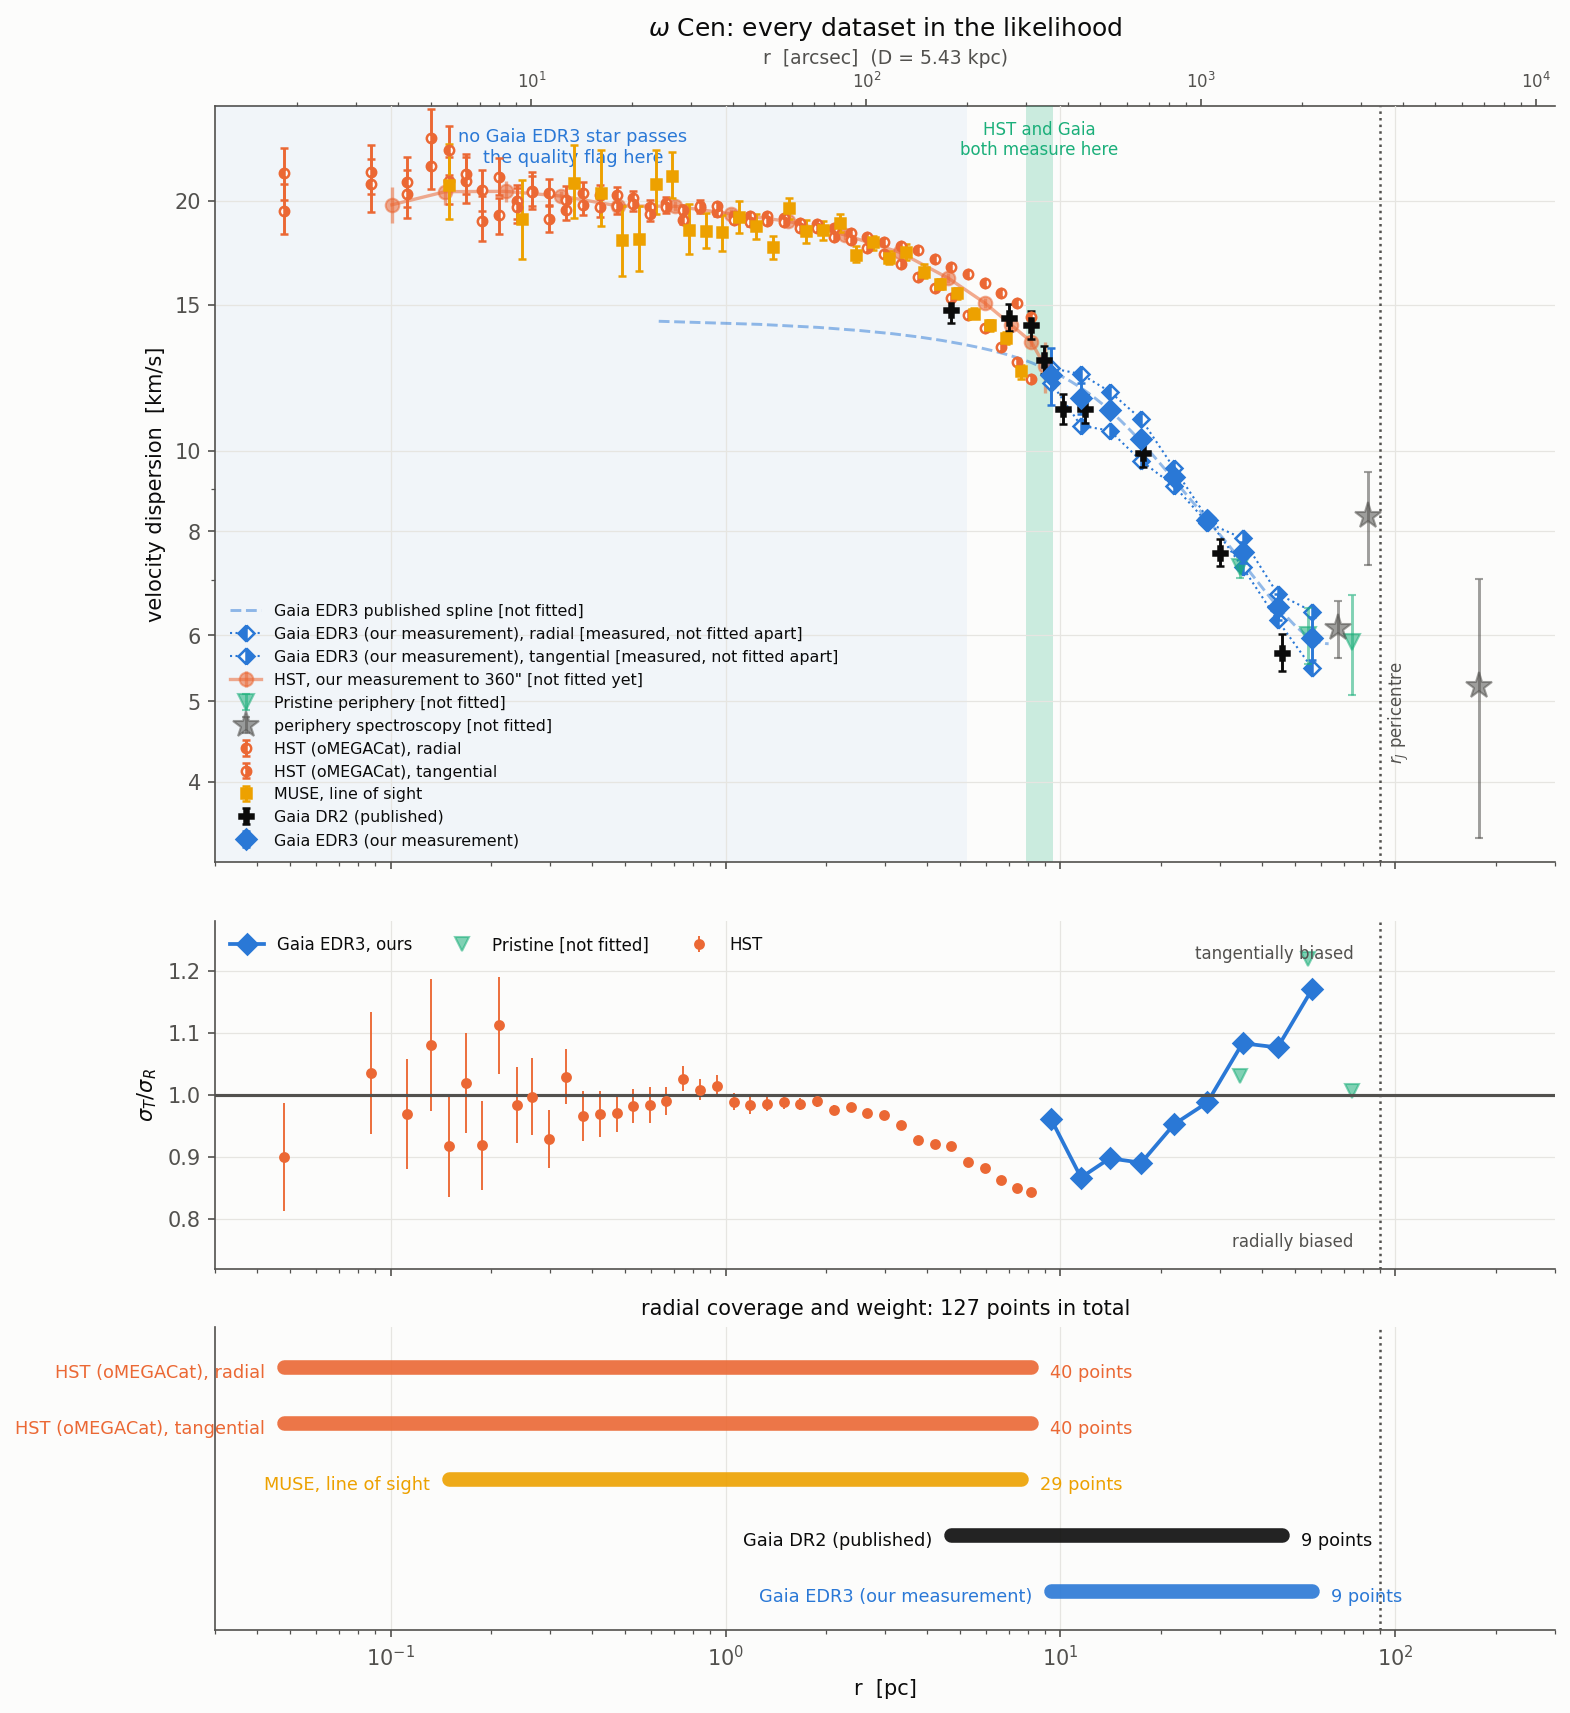
\includegraphics[width=0.92\textwidth]{master_datasets.png}
\caption{Every dataset in the likelihood, converted to \kms\ at $D=5.43$\,kpc so that proper
motions and line-of-sight velocities share an axis. One symbol and colour per dataset
throughout; the radial and tangential components of the same stars share that symbol and are
distinguished by the marker fill. Middle: the anisotropy implied by those components. Bottom:
radial coverage and point count.}
\end{figure}

\begin{figure}[p]
\centering
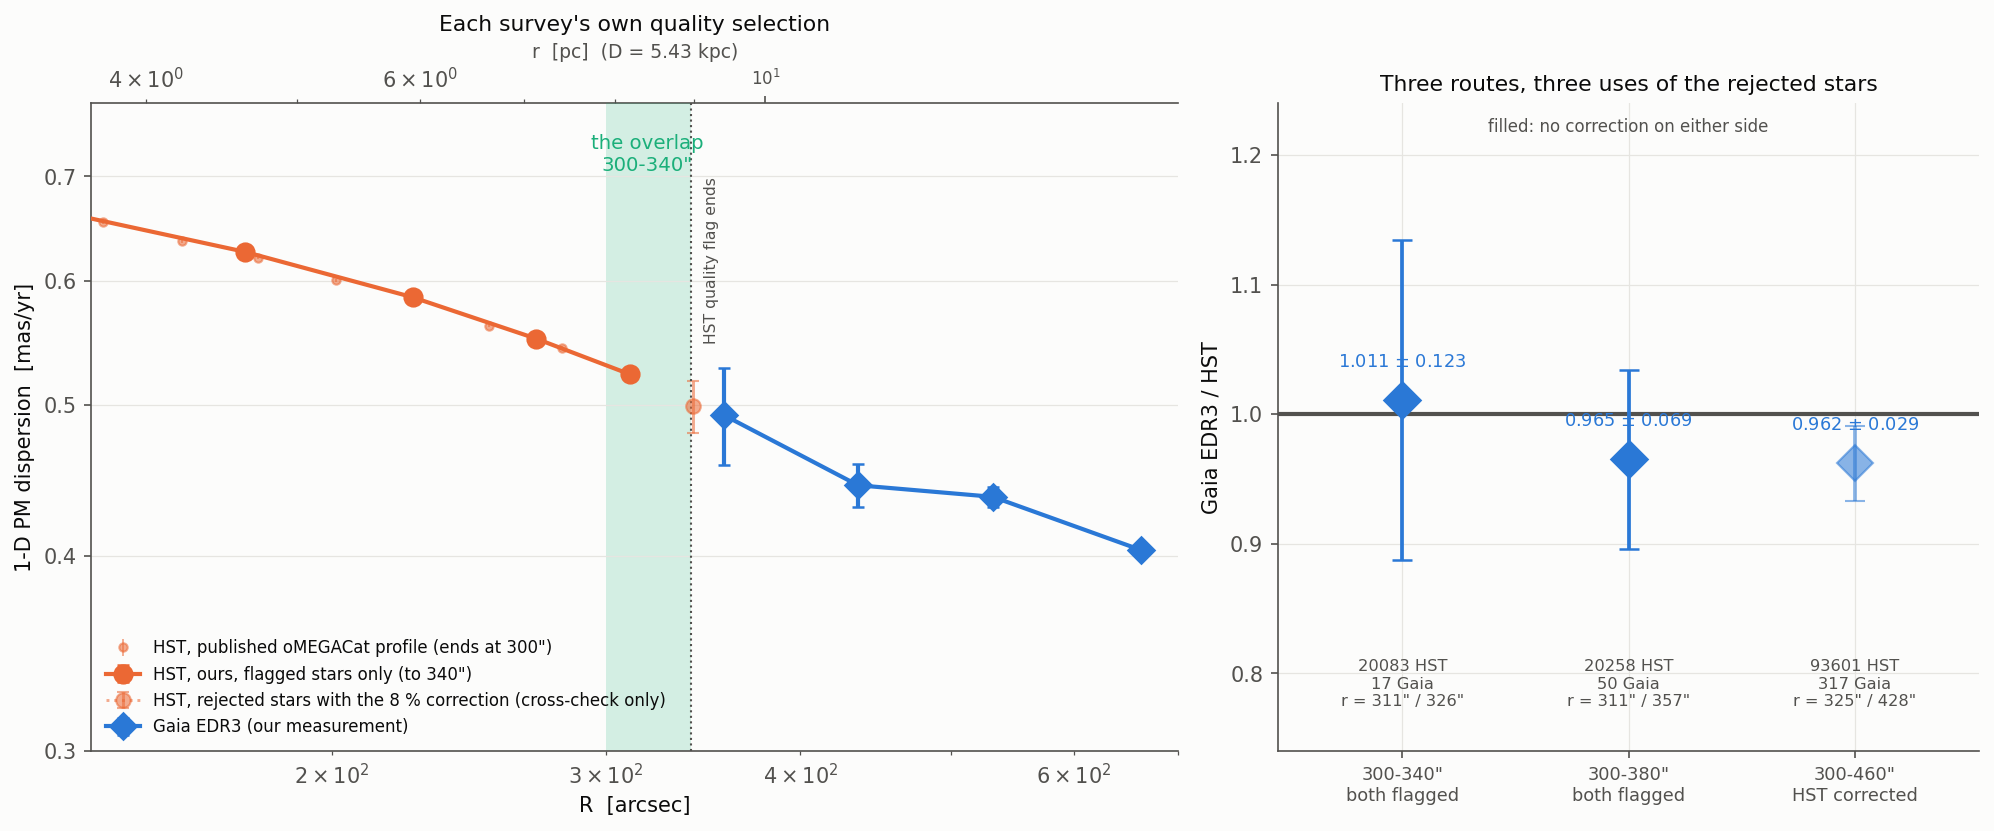
\includegraphics[width=0.98\textwidth]{hst_gaia_overlap.png}
\caption{Left: HST measured from its own flagged stars, which reaches $360''$, against
\emph{Gaia}, which starts at $300''$. The published oMEGACat profile, which stops at $300''$,
is shown faintly. Right: the comparison by three routes differing in their use of HST's
rejected stars.}
\end{figure}

\begin{figure}[p]
\centering
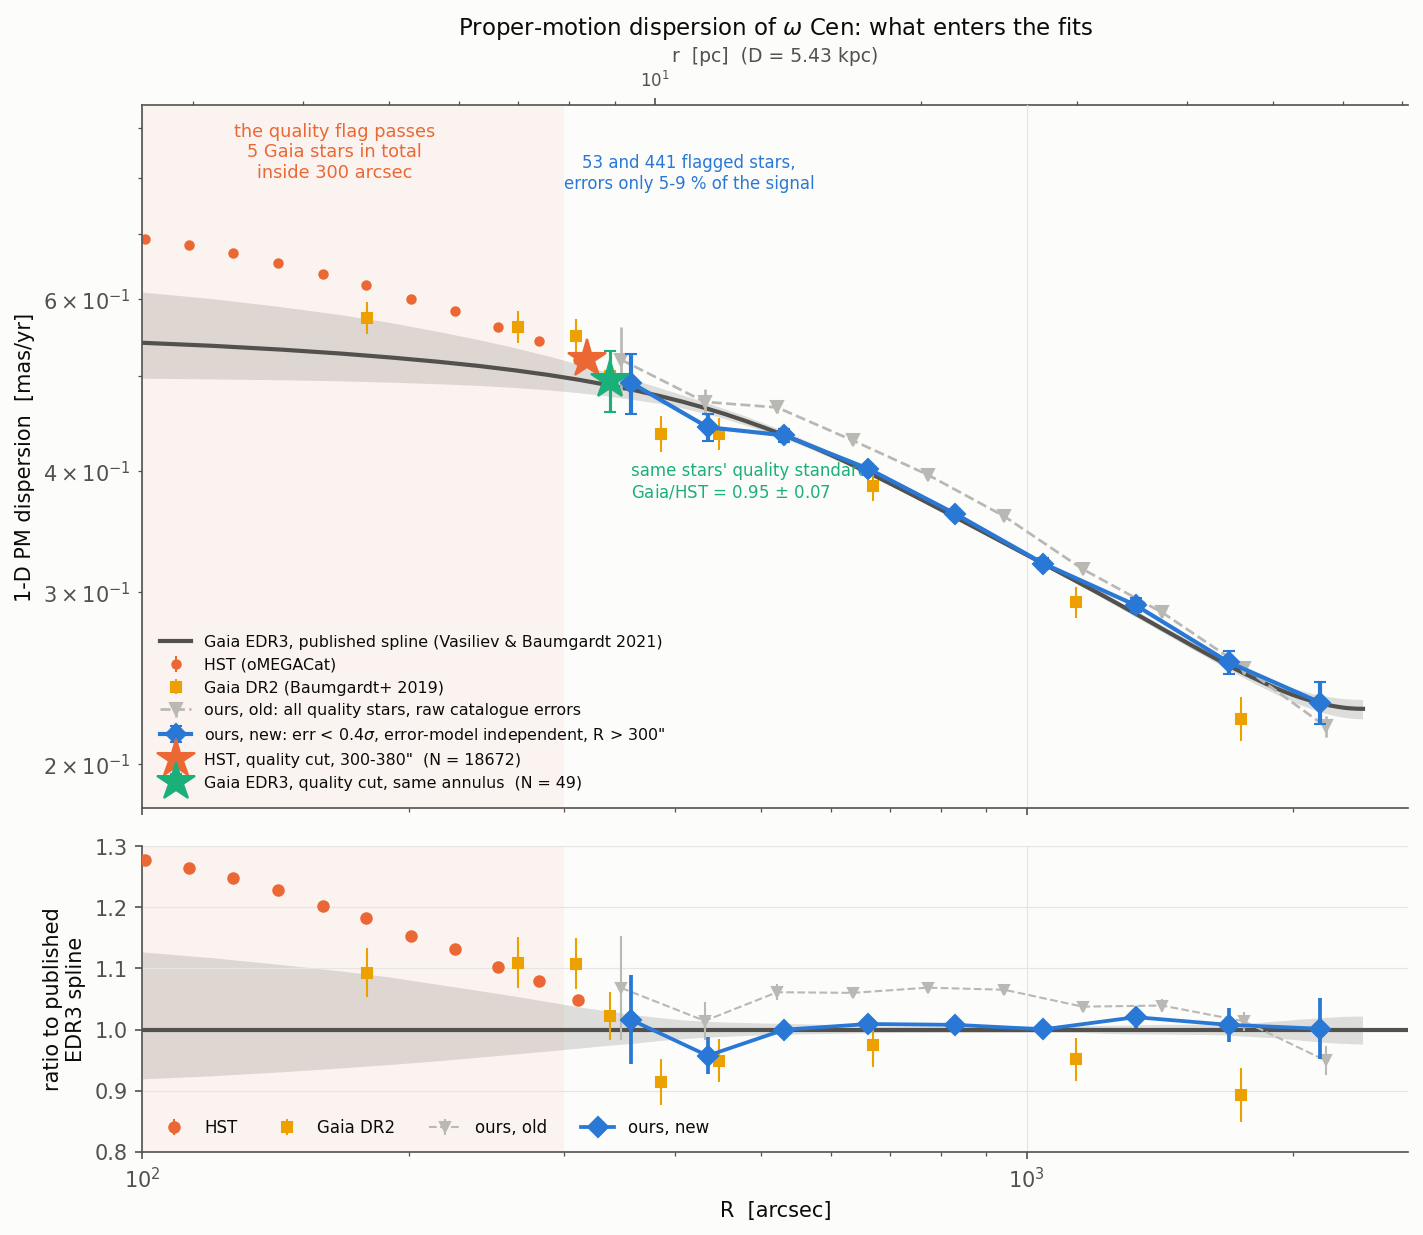
\includegraphics[width=0.98\textwidth]{pm_datasets_edr3_rebuild.png}
\caption{The rebuilt \emph{Gaia} EDR3 measurement against the published spline and against
our earlier version, which deconvolved the raw catalogue errors and ran 4--7 per cent high.
The lower panel is the ratio to the published spline.}
\end{figure}

\begin{figure}[p]
\centering
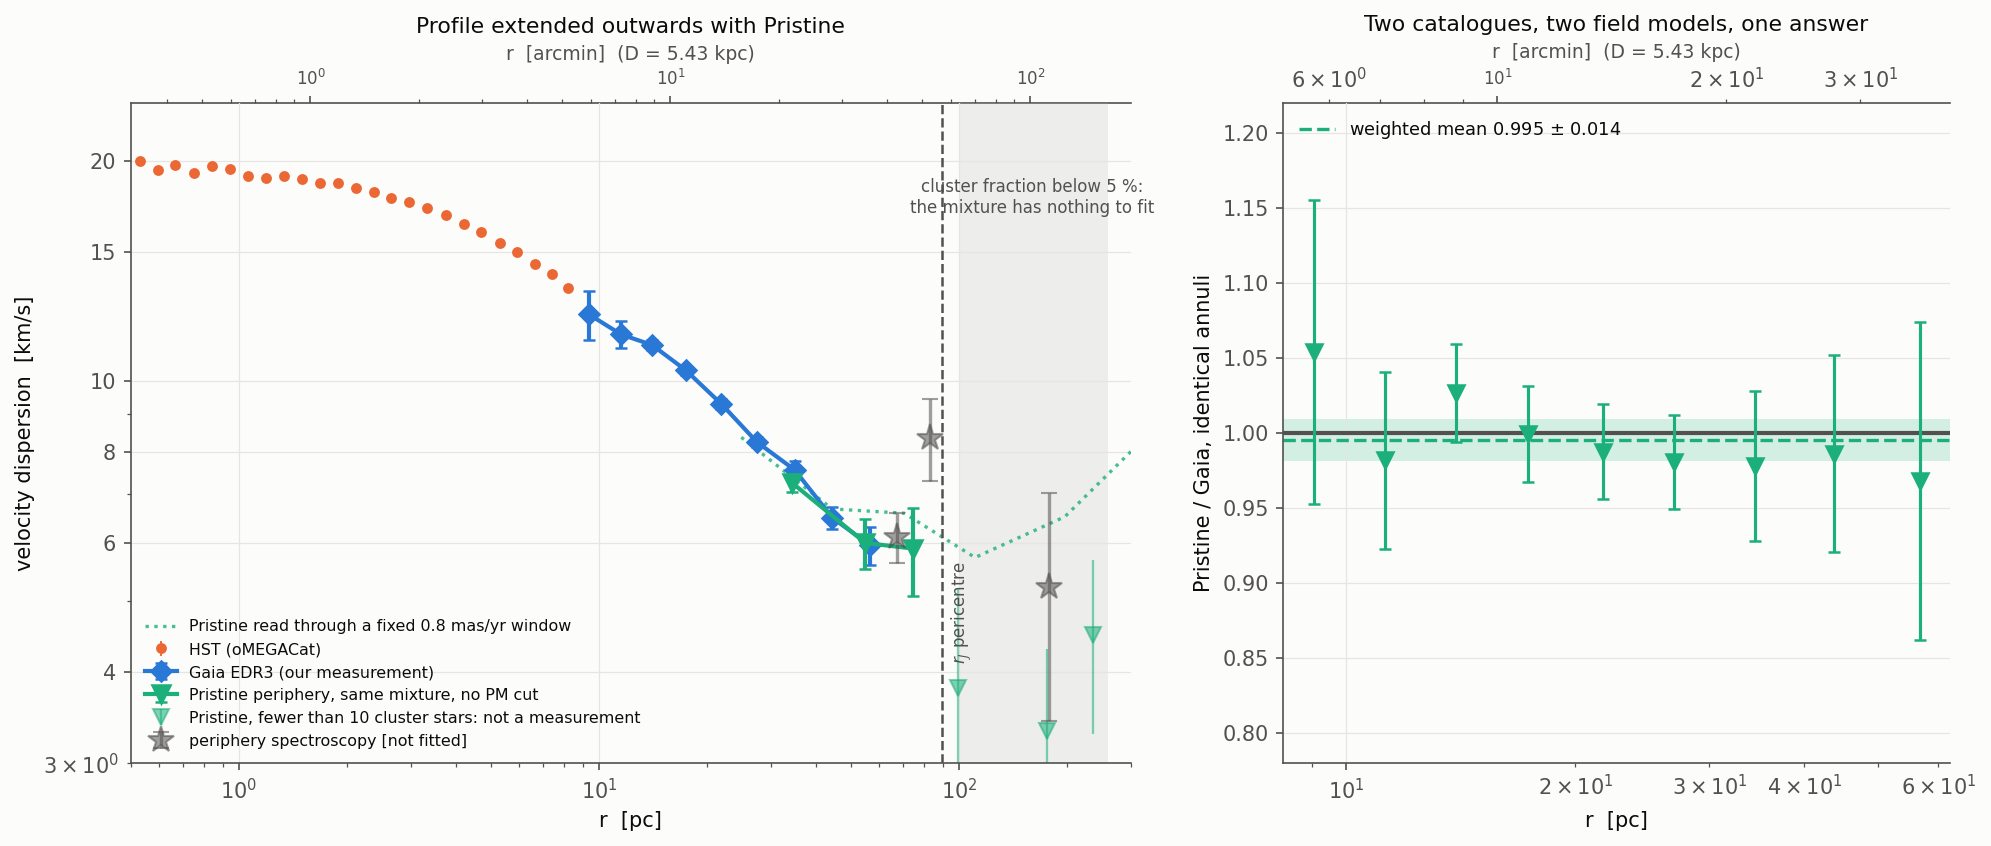
\includegraphics[width=0.98\textwidth]{profile_extended_pristine.png}
\caption{Left: the profile extended outwards with Pristine through the same mixture, with no
proper-motion selection, against the same catalogue read through a fixed window. Right:
Pristine over \emph{Gaia} on identical annuli, $0.995\pm0.014$.}
\end{figure}

\begin{figure}[p]
\centering
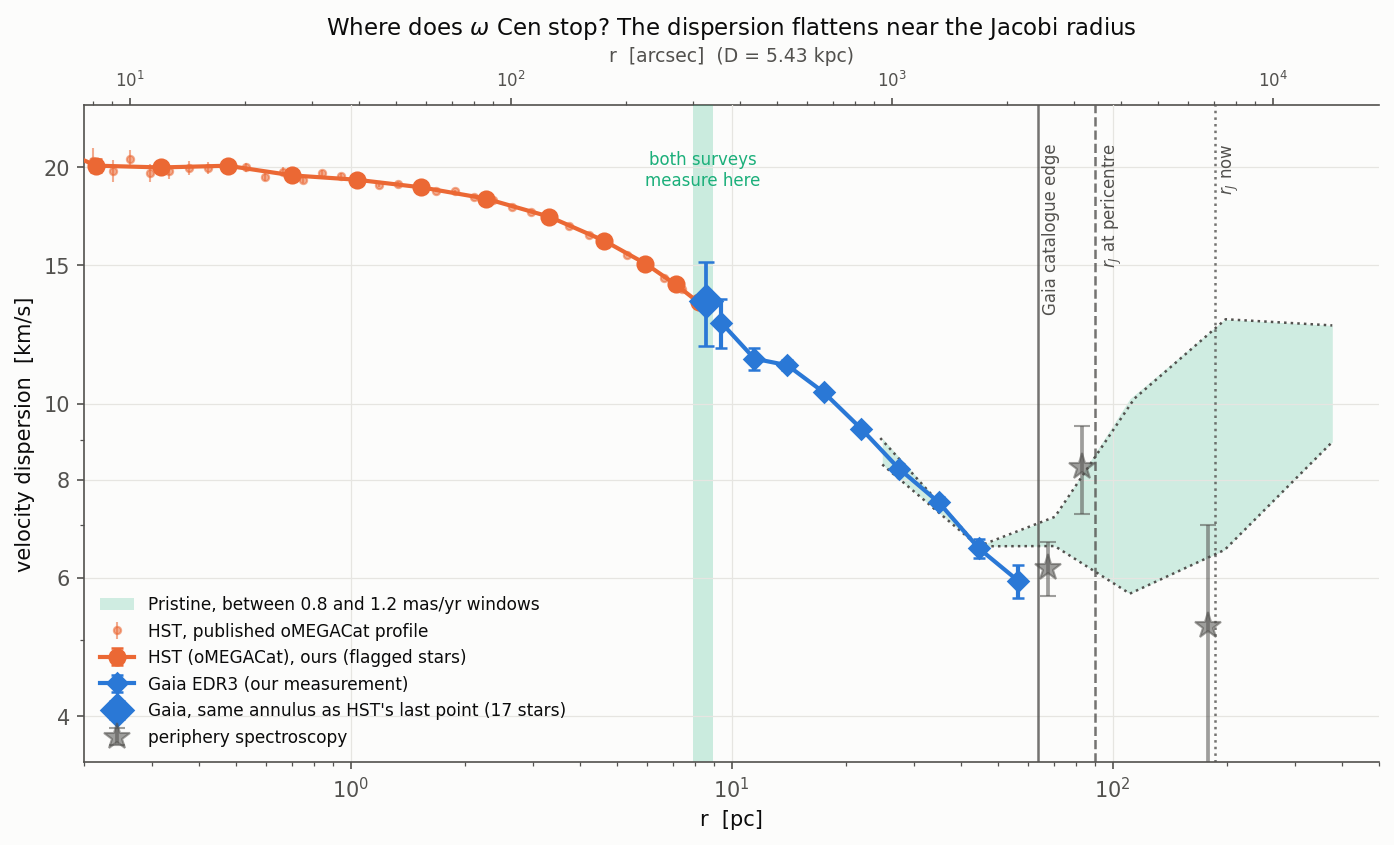
\includegraphics[width=0.92\textwidth]{periphery_where_the_cluster_ends.png}
\caption{The profile from the centre to 400\,pc. The dispersion stops falling near
$50$--$100$\,pc, where the pericentric Jacobi radius lies.}
\end{figure}

\begin{figure}[p]
\centering
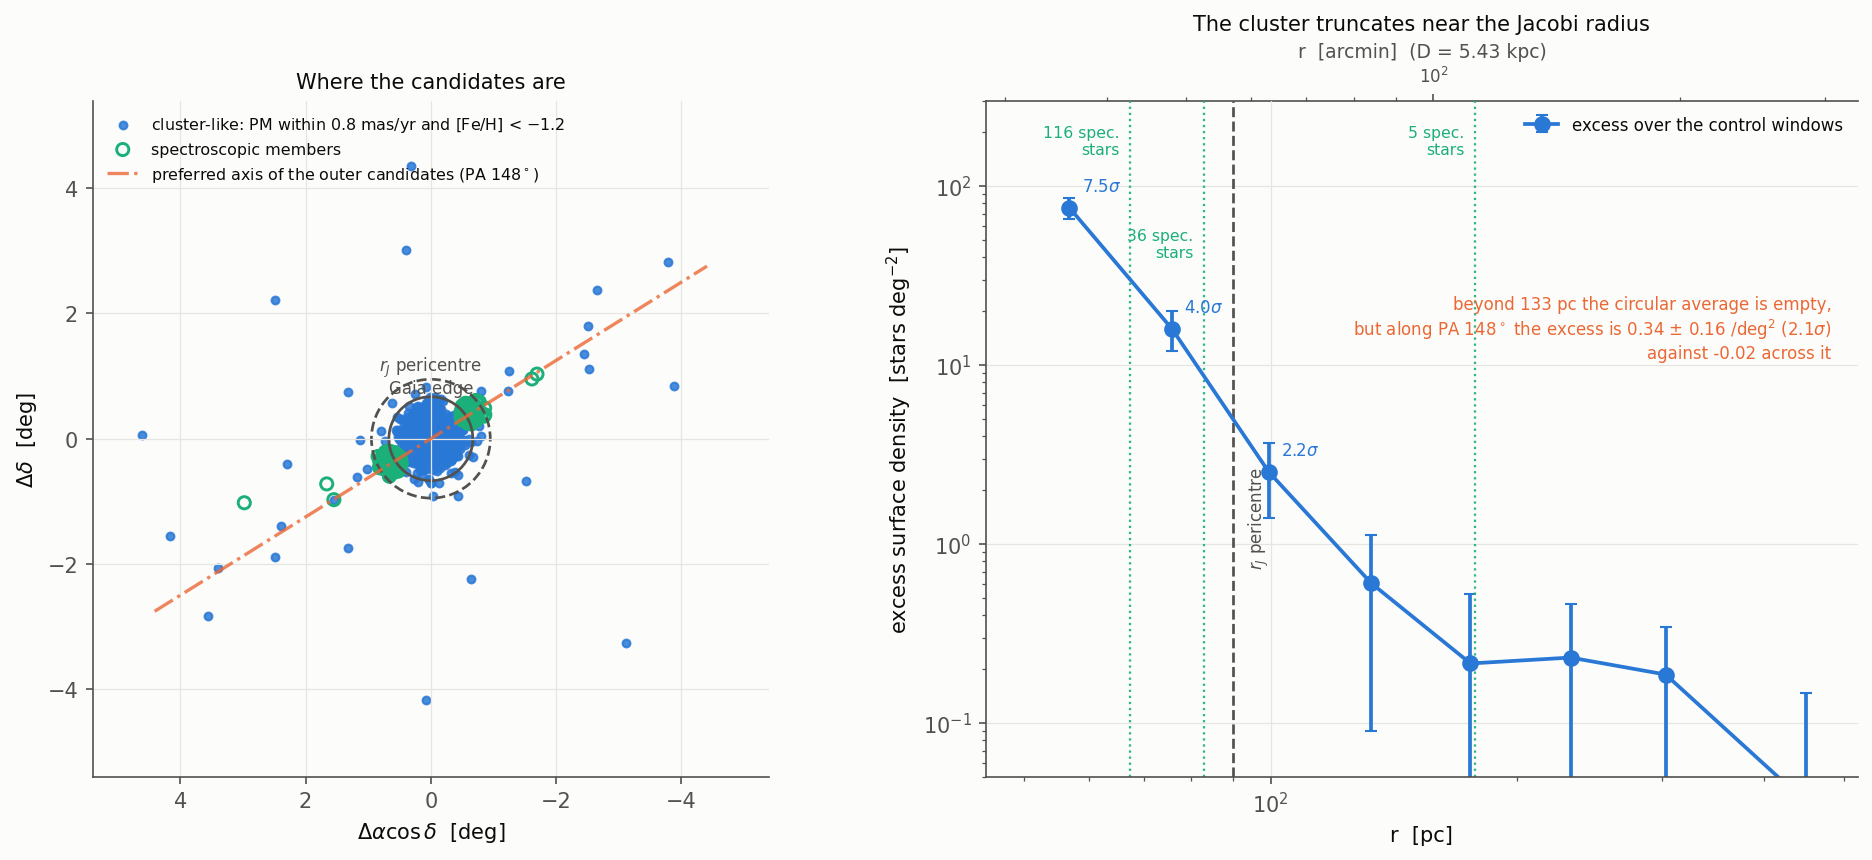
\includegraphics[width=0.98\textwidth]{periphery_overdensity.png}
\caption{Left: cluster-like stars on the sky, selected on proper motion and CaHK metallicity,
with the spectroscopic members overplotted. Right: their background-subtracted surface
density, truncating near the Jacobi radius.}
\end{figure}

\begin{thebibliography}{9}
\bibitem[Baumgardt et al.(2019)]{baumgardt2019} Baumgardt, H., Hilker, M., Sollima, A.,
  Bellini, A. 2019, MNRAS, 482, 5138.
  \url{https://ui.adsabs.harvard.edu/abs/2019MNRAS.482.5138B}
\bibitem[H\"aberle et al.(2025)]{haeberle2025} H\"aberle, M., Neumayer, N., Clontz, C.,
  et al. 2025, ApJ, \emph{oMEGACat VI}. \url{https://arxiv.org/abs/2503.04903},
  \url{https://doi.org/10.3847/1538-4357/adbe67}
\bibitem[Kuzma \& Ishigaki(2025)]{kuzma2025} Kuzma, P. B., Ishigaki, M. N. 2025, MNRAS, 537,
  2752. \url{https://arxiv.org/abs/2502.01135},
  data \url{https://doi.org/10.5281/zenodo.14791430}
\bibitem[Kuzma et al.(2026)]{kuzma2026} Kuzma, P. B., et al. 2026, MNRAS, 550,
  \emph{Disruption of a Giant}. \url{https://arxiv.org/abs/2605.23474}
\bibitem[Vasiliev \& Baumgardt(2021)]{vasiliev2021} Vasiliev, E., Baumgardt, H. 2021, MNRAS,
  505, 5978. \url{https://arxiv.org/abs/2102.09568}
\bibitem[Vasiliev et al.(2020)]{vasiliev2020} Vasiliev, E., Belokurov, V., Erkal, D. 2020,
  MNRAS, 501, 2279. \url{https://arxiv.org/abs/2009.10726}
\end{thebibliography}

\end{document}
